\documentclass[border=10pt]{standalone}
\usepackage{tikz}
\usetikzlibrary{hobby}
\definecolor{myred}{RGB}{190,60,45}
\definecolor{myblue}{RGB}{38,84,160}

\begin{document}
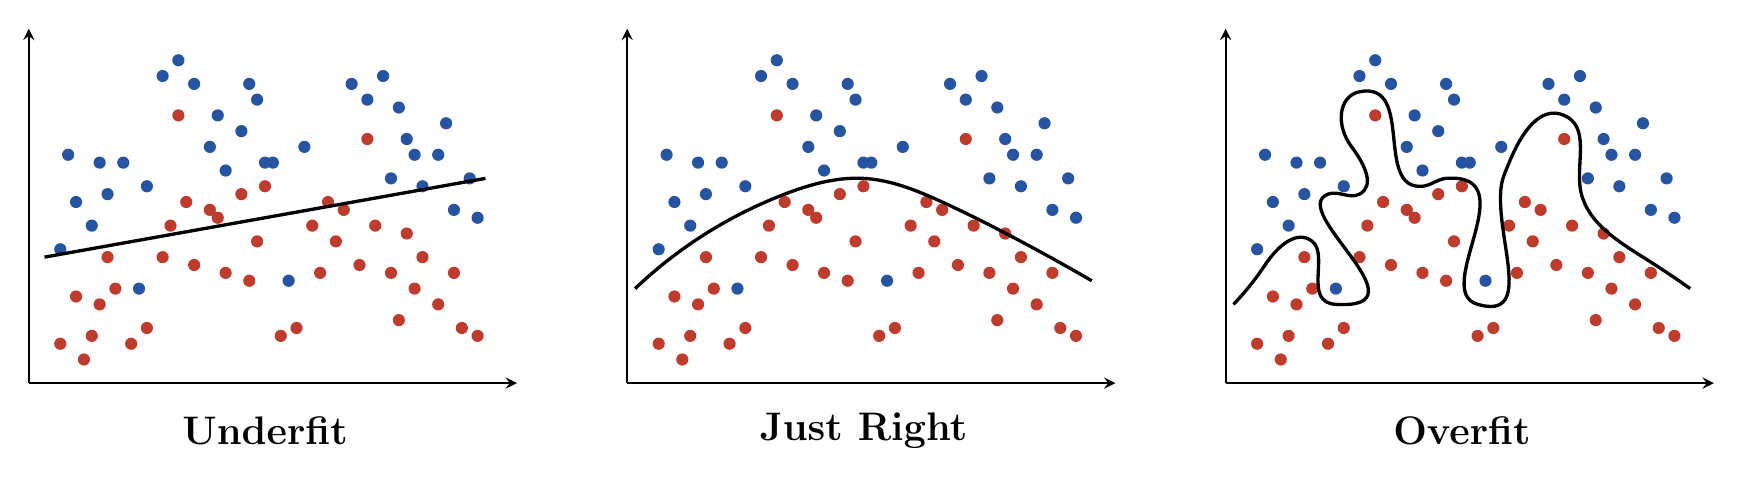
\begin{tikzpicture}[>=stealth, line width=0.8pt, font=\large]
  % 增加点数，缩小红蓝集团的间距，形成一个明显的"拱形(抛物线)"间隙
  % 真实边界大致围绕 y = -0.15(x-3)^2 + 2.5 左右
  
  % === 红类 (主集团位于拱形下方) ===
  \def\redpts{
    % 正常点 (密集分布在拱形下方)
    0.4/0.5, 0.6/1.1, 0.8/0.6, 1.0/1.6, 1.1/1.2, 1.3/0.5, 1.5/0.7, 
    1.7/1.6, 1.8/2.0, 2.0/2.3, 2.1/1.5, 2.3/2.2, 2.5/1.4, 2.7/2.4, 
    2.9/1.8, 3.0/2.5, 3.2/0.6, 3.4/0.7, 3.6/2.0, 3.8/2.3, 4.0/2.2, 
    4.2/1.5, 4.4/2.0, 4.6/1.4, 4.8/1.9, 5.0/1.6, 5.2/1.0, 5.4/1.4, 5.7/0.6,
    0.7/0.3, 0.9/1.0, 2.4/2.1, 2.8/1.3, 3.7/1.4, 3.9/1.8, 4.7/0.8, 4.9/1.2, 5.5/0.7,
    % 2个噪声点 (极其突兀地跑到蓝类的上方)
    1.9/3.4, 4.3/3.1
  }
  
  % === 蓝类 (主集团位于拱形上方) ===
  \def\bluepts{
    % 正常点 (密集分布在拱形上方)
    0.4/1.7, 0.6/2.3, 0.8/2.0, 1.0/2.4, 1.2/2.8, 1.5/2.5, 
    1.7/3.9, 1.9/4.1, 2.1/3.8, 2.3/3.0, 2.5/2.7, 2.7/3.2, 
    2.9/3.6, 3.0/2.8, 3.1/2.8, 3.5/3.0, 4.1/3.8, 4.3/3.6, 
    4.5/3.9, 4.6/2.6, 4.8/3.1, 5.0/2.5, 5.2/2.9, 5.4/2.2, 5.6/2.6,
    0.5/2.9, 0.9/2.8, 2.4/3.4, 2.8/3.8, 4.7/3.5, 4.9/2.9, 5.3/3.3, 5.7/2.1,
    % 2个噪声点 (极其突兀地掉到红类的下方)
    1.4/1.2, 3.3/1.3
  }
  
  \newcommand{\drawpts}{%
    \foreach \x/\y in \redpts  \fill[myred]  (\x,\y) circle (2.2pt);
    \foreach \x/\y in \bluepts \fill[myblue] (\x,\y) circle (2.2pt);
  }

  % ===== 1 underfit：用直线去切拱形，导致大片错误 =====
  \begin{scope}[xshift=0cm]
    \draw[->] (0,0) -- (6.2,0); \draw[->] (0,0) -- (0,4.5);
    \drawpts
    % 直线强行切过去：中间红点（高于2.1）被误判，右侧蓝点（低于2.4）被误判
    \draw[black, line width=1.2pt] (0.2, 1.6) -- (5.8, 2.6);
    \node[font=\Large\bfseries] at (3,-0.6) {Underfit};
  \end{scope}

  % ===== 2 just right：平滑拱形，穿过缝隙，果断忽略噪声 =====
  \begin{scope}[xshift=7.6cm]
    \draw[->] (0,0) -- (6.2,0); \draw[->] (0,0) -- (0,4.5);
    \drawpts
    % 完美的平滑曲线，紧密贴合真实的类间间隙
    \draw[black, line width=1.2pt] (0.1, 1.2) 
      to[curve through={(1.0, 1.9) (2.0, 2.4) (3.0, 2.6) (4.0, 2.3) (5.0, 1.8)}] (5.9, 1.3);
    \node[font=\Large\bfseries] at (3,-0.6) {Just Right};
  \end{scope}

  % ===== 3 overfit：蛇形走位，强行折返包裹每一个噪声 =====
  \begin{scope}[xshift=15.2cm]
    \draw[->] (0,0) -- (6.2,0); \draw[->] (0,0) -- (0,4.5);
    \drawpts
    % 为了4个噪声点，疯狂上下拉扯出“触角”
    \draw[black, line width=1.2pt] (0.1, 1.0) 
      to[curve through={
        (0.5, 1.5) 
        (1.1, 1.8) 
        (1.4, 1.0) % 向下深挖：包裹蓝噪声 (1.4, 1.2)
        (1.3, 2.4) 
        (1.7, 2.4) 
        (1.6, 3.0) 
        (1.7, 3.7) % 向上拉刺：包裹红噪声 (1.9, 3.4)
        (2.5, 2.5) 
        (2.8, 2.6) 
        (3.2, 1.0) % 向下深挖：包裹蓝噪声 (3.3, 1.3)
        (3.5, 2.5) 
        (3.6, 2.8) 
        (4.3, 3.4) % 向上拉刺：包裹红噪声 (4.3, 3.1)
        (4.5, 2.5) 
        (5.3, 1.6)
      }] (5.9, 1.2);
    \node[font=\Large\bfseries] at (3,-0.6) {Overfit};
  \end{scope}
\end{tikzpicture}
\end{document}